\documentclass{class/tum_report}

\usepackage{booktabs}
\usepackage{tabularx}
\usepackage{longtable}
\usepackage{microtype}
\let\tumyear\year
\ExplSyntaxOn
\cs_set_eq:NN \year \tex_year:D
\ExplSyntaxOff
\usepackage{pgfplots}
\pgfplotsset{compat=1.18}
\usetikzlibrary{arrows.meta, positioning, fit, backgrounds, calc}
\let\year\tumyear

\geometry{a4paper, top=2cm, bottom=2cm, left=2cm, right=2cm}

\titleclass{\chapter}{straight}
\titlespacing*{\chapter}{0pt}{16pt}{4pt}
\setlength{\textfloatsep}{12pt plus 2pt minus 2pt}
\setlength{\intextsep}{10pt plus 2pt minus 2pt}
\newcommand{\tocchapter}[1]{\chapter*{#1}\phantomsection\addcontentsline{toc}{chapter}{#1}\nobreak}

\definecolor{natclassic}{HTML}{3B6EA8}
\definecolor{nathybrid}{HTML}{D9952B}
\definecolor{natnative}{HTML}{B8475A}
\definecolor{softgray}{HTML}{6B7280}
\hypersetup{colorlinks=true, linkcolor=black, citecolor=natclassic, urlcolor=natclassic}

\newacronym[description={Application Programming Interface. A defined way for one program to request data or actions from another, usually over HTTP}]{glo:api}{API}{Application Programming Interface}
\newacronym[description={Common Vulnerabilities and Exposures. A public catalogue that gives each confirmed security flaw in a specific product a unique identifier, for example CVE-2025-6514}]{glo:cve}{CVE}{Common Vulnerabilities and Exposures}
\newacronym[description={Common Vulnerability Scoring System. A 0 to 10 scale used to rate the severity of a vulnerability; scores of 9.0 and above are considered critical}]{glo:cvss}{CVSS}{Common Vulnerability Scoring System}
\newacronym[description={Personal identification number (Numărul de identificare de stat). The 13-digit number assigned to every citizen of the Republic of Moldova and used as the key in state registries}]{glo:idnp}{IDNP}{personal identification number}
\newacronym[description={Large Language Model. A neural network trained on large amounts of text that generates answers and, in agent systems, decides which tools to call}]{glo:llm}{LLM}{Large Language Model}
\newacronym[description={Model Context Protocol. An open standard, published in 2024, that defines how AI applications discover and call external tools and data sources}]{glo:mcp}{MCP}{Model Context Protocol}
\newacronym[description={Remote Code Execution. A vulnerability that lets an attacker run their own commands on another machine, usually the most severe outcome of an attack}]{glo:rce}{RCE}{Remote Code Execution}
\newacronym[description={Software Development Kit. A library provided by the protocol maintainers that developers use to build servers and clients}]{glo:sdk}{SDK}{Software Development Kit}
\newacronym[description={Server-Side Request Forgery. A flaw that makes a server send requests to addresses chosen by the attacker, often internal services or cloud metadata endpoints}]{glo:ssrf}{SSRF}{Server-Side Request Forgery}
\newacronym[description={Vulnerable MCP Project. An openly maintained online catalogue of documented MCP weaknesses, used as the main data source of this study}]{glo:vmp}{VMP}{Vulnerable MCP Project}

\newcommand{\nRecords}{54}
\newcommand{\nVmp}{49}
\newcommand{\nSupplementary}{5}
\newcommand{\nClassic}{33}
\newcommand{\pClassic}{61.1}
\newcommand{\nHybrid}{5}
\newcommand{\pHybrid}{9.3}
\newcommand{\nNative}{16}
\newcommand{\pNative}{29.6}
\newcommand{\nCve}{20}
\newcommand{\pCve}{37.0}
\newcommand{\nCveClassic}{19}
\newcommand{\nCveHybrid}{1}
\newcommand{\nCveNative}{0}
\newcommand{\pClassicWithCve}{57.6}
\newcommand{\nFirstParty}{8}
\newcommand{\nFirstPartyClassic}{7}
\newcommand{\nInsecureDefault}{9}
\newcommand{\pInsecureDefaultOfClassic}{27.3}
\newcommand{\nImplClassic}{27}
\newcommand{\pImplClassic}{50.0}
\newcommand{\pClassicComma}{61,1}
\newcommand{\pNativeComma}{29,6}
\newcommand{\ciClassicLow}{47.8}
\newcommand{\ciClassicHigh}{73.0}
\newcommand{\nCommandInjection}{7}
\newcommand{\nPathTraversal}{6}
\newcommand{\nSsrf}{3}
\newcommand{\nAccessControl}{9}
\newcommand{\nMainFamilies}{25}
\newcommand{\nMaliciousPackage}{2}
\newcommand{\nNativeViaServer}{10}
\newcommand{\nNativeViaContent}{6}
\newcommand{\nNativeProtocol}{11}
\newcommand{\nNativeIntegration}{4}
\newcommand{\nIntegration}{5}
\newcommand{\nServer}{20}
\newcommand{\nServerCve}{12}
\newcommand{\firstDisclosure}{March 2025}
\newcommand{\lastDisclosure}{February 2026}

\pgfplotsset{quarteraxis/.style={symbolic x coords={2025 Q1,2025 Q2,2025 Q3,2025 Q4,2026 Q1}}}
\newcommand{\quarterPlots}{%
\addplot coordinates {(2025 Q1,1) (2025 Q2,5) (2025 Q3,13) (2025 Q4,5) (2026 Q1,9)};
\addlegendentry{Classic}
\addplot coordinates {(2025 Q1,0) (2025 Q2,2) (2025 Q3,1) (2025 Q4,2) (2026 Q1,0)};
\addlegendentry{Hybrid}
\addplot coordinates {(2025 Q1,0) (2025 Q2,11) (2025 Q3,2) (2025 Q4,3) (2026 Q1,0)};
\addlegendentry{AI-native}
}

\def\cveWithClassic{19}
\def\cveWithoutClassic{14}
\def\cveWithHybrid{1}
\def\cveWithoutHybrid{4}
\def\cveWithAInative{0}
\def\cveWithoutAInative{16}


\begin{document}

    \renewcommand{\glossaryname}{List of abbreviations}

    \ministry{Ministry of Education and Research of the Republic of Moldova}
\university{Technical University of Moldova}
\faculty{Faculty of Computers, Informatics and Microelectronics}
\department{Department of Software Engineering and Automatics}

\title{Old Bugs, New Protocol: A Root-Cause Analysis of Security Failures in the Model Context Protocol Ecosystem Under Rapid Adoption}{Erori vechi, protocol nou: analiza cauzelor eșecurilor de securitate din ecosistemul Model Context Protocol în condițiile adoptării accelerate}

\year{2026}


\begin{titlepage}

    {\MakeUppercase{\ministryname} \par}
    \vspace{0.2cm}
    {\large \universityname \par}
    {\large \facultyname \par}
    {\large \departmentname \par}

	\vfill

	{\LARGE \titleen \par}
	\vspace{0.5cm}
	{\large \mdseries \itshape \titlero \par}
	\vspace{1cm}
	{\Large Research article \par}
	\vspace{0.2cm}
	{\large \mdseries Master programme: Software Engineering \par}

	\vfill

    \begin{table}[h!]
        \hfill
        \begin{tabular}{ll}
        \textbf{Student:}    & Negai Marin, group IS-261M \\[0.3cm]
        \textbf{Supervisor:} & \rule{6.5cm}{0.4pt} \\
        \end{tabular}
    \end{table}

	\vfill

	{\large Chișinău, \degreeyear \par}

\end{titlepage}

    \clearpage

    \chapter*{Abstract}

\par Negai Marin, \textit{``Old Bugs, New Protocol: A Root-Cause Analysis of Security Failures in the Model Context Protocol Ecosystem Under Rapid Adoption''}, research article, Technical University of Moldova, Faculty of Computers, Informatics and Microelectronics, Chișinău, 2026. The article has an introduction, four chapters, conclusions, a bibliography of 30 sources and one appendix. It contains 5 figures and 5 tables.

\vspace{0.3cm}
\par \noindent \textbf{Keywords:} Model Context Protocol, AI agents, software security, prompt injection, vulnerability analysis.
\vspace{0.3cm}

\par The Model Context Protocol (MCP) was released at the end of 2024 as a common way to connect language-model assistants to files, databases and online services. Within a year it was supported by most large AI vendors, and during the same period security researchers published dozens of reports about vulnerable servers, compromised packages and attacks that hide instructions inside tool descriptions. These reports are usually discussed as a new ``AI security'' problem. The question behind this article is whether that label is accurate, or whether most of the failures are ordinary software defects that appeared because the ecosystem grew faster than anyone could review it.

\par The objective was to find where MCP security failures come from. I collected \nRecords{} publicly documented weaknesses and incidents disclosed between \firstDisclosure{} and \lastDisclosure{}, mainly from an open vulnerability catalogue and partly from the original research disclosures. Every record was read in its original source and coded on two axes. The first axis is the nature of the flaw: classic (it would exist even without a language model), AI-native (it works only because a model follows text it should not trust) or hybrid. The second axis is the stage where the flaw was introduced: protocol design, implementation, integration design, supply chain or deployment. All counts and charts were produced by a small Python script from the coded dataset, which is published together with the article.

\par The results show that \pClassic\% of the records are classic weaknesses such as command injection, path traversal, server-side request forgery and missing authentication, and half of all records are coding mistakes in individual servers, clients or tools. AI-native weaknesses make up \pNative\% of the sample and come almost entirely from the design of the protocol and of the integrations built on it. None of them received a CVE identifier, which means that tools based on vulnerability databases cannot see this part of the risk. The article ends with a set of controls for developers, operators and public institutions, and compares the findings with the October 2026 breach of Moldovan e-government services, where a comparable trust error led to the exposure of personal data of about 450,000 citizens.

    \clearpage

    \chapter*{Adnotare}

\par Negai Marin, \textit{``Erori vechi, protocol nou: analiza cauzelor eșecurilor de securitate din ecosistemul Model Context Protocol în condițiile adoptării accelerate''}, articol științific, Universitatea Tehnică a Moldovei, Facultatea Calculatoare, Informatică și Microelectronică, Chișinău, 2026. Articolul este alcătuit din introducere, patru capitole, concluzii, o bibliografie din 30 de surse și o anexă. Lucrarea conține 5 figuri și 5 tabele.

\vspace{0.3cm}
\par \noindent \textbf{Cuvinte-cheie:} Model Context Protocol, agenți AI, securitate software, injectare de prompt, analiza vulnerabilităților.
\vspace{0.3cm}

\par Model Context Protocol (MCP) a fost lansat la sfârșitul anului 2024 ca o modalitate comună de a conecta asistenții bazați pe modele de limbaj la fișiere, baze de date și servicii online. În decurs de un an, protocolul a fost preluat de majoritatea companiilor mari din domeniul AI, iar cercetătorii au publicat zeci de rapoarte despre servere vulnerabile și atacuri care ascund instrucțiuni în descrierile instrumentelor. Aceste probleme sunt prezentate de obicei ca un risc nou, specific AI. Articolul verifică dacă această interpretare este corectă sau dacă majoritatea eșecurilor sunt defecte software obișnuite, apărute pentru că ecosistemul a crescut mai repede decât a putut fi verificat.

\par Obiectivul lucrării a fost identificarea surselor eșecurilor de securitate din MCP. Au fost colectate \nRecords{} de vulnerabilități și incidente documentate public, dezvăluite între martie 2025 și februarie 2026, dintr-un catalog deschis de vulnerabilități și din publicațiile originale. Fiecare înregistrare a fost citită în sursa originală și clasificată pe două axe. Prima axă descrie natura defectului: clasic (ar exista și fără un model de limbaj), specific AI (funcționează doar pentru că modelul urmează un text în care nu ar trebui să aibă încredere) sau hibrid. A doua axă indică etapa în care a apărut defectul: proiectarea protocolului, implementarea, proiectarea integrării, lanțul de aprovizionare sau configurarea la instalare. Toate valorile au fost calculate de un script Python pe baza setului de date publicat.

\par Rezultatele arată că \pClassicComma\% dintre înregistrări sunt vulnerabilități clasice, precum injectarea de comenzi, traversarea căilor, falsificarea cererilor din partea serverului și lipsa autentificării, iar jumătate din totalul înregistrărilor sunt greșeli de programare în servere, clienți sau instrumente. Vulnerabilitățile specifice AI reprezintă \pNativeComma\% din eșantion și provin aproape în totalitate din proiectarea protocolului și a integrărilor. Niciuna dintre ele nu a primit un identificator CVE, deci instrumentele bazate pe baze de date de vulnerabilități nu pot observa această parte a riscului. Articolul propune un set de măsuri pentru dezvoltatori, operatori și instituții publice și compară rezultatele cu incidentul din octombrie 2026 care a afectat serviciile de guvernare electronică din Republica Moldova, unde o eroare de încredere asemănătoare a dus la expunerea datelor personale a aproximativ 450.000 de cetățeni.

    \clearpage

    \addtocontents{toc}{\protect \thispagestyle{empty}}
    \tableofcontents
    \thispagestyle{empty}
    \clearpage

    \addcontentsline{toc}{chapter}{\glossaryname}
    \printnoidxglossary[type=\acronymtype, nogroupskip, nonumberlist, style=myGlossaryStyle]
    \thispagestyle{empty}
    \clearpage

    \tocchapter{Introduction}

\par Over the last two years, AI assistants have moved from answering questions to performing tasks. A coding assistant now opens files, runs tests and creates pull requests; an office assistant reads the mailbox and books meetings. To do this, the model needs a way to reach external systems. Until late 2024 every vendor built its own connectors. In November 2024 Anthropic published the \acrfull{glo:mcp}, an open specification that describes how an AI application finds the tools offered by an external program and how it calls them \cite{anthropic2024mcp}. The protocol was adopted quickly. OpenAI and Google announced support in the spring of 2025, and in December 2025 the project was transferred to the Agentic AI Foundation, which operates under the Linux Foundation \cite{aaif2025}. In July 2026 Netskope reported that \acrshort{glo:mcp} traffic among its customers had grown four times in only ten weeks \cite{netskope2026}.

\par The security of the ecosystem developed more slowly. The first version of the specification did not include any authorisation mechanism. Critical vulnerabilities were found in official reference servers and in the developer tools published by the maintainers, and internet-wide scans in 2026 found thousands of servers that accepted requests without checking who sent them \cite{zhou2026, padilla2026}. In May 2026 the U.S. National Security Agency released a separate information sheet on the secure use of \acrshort{glo:mcp} \cite{nsa2026}.

\par In public discussion these problems are usually grouped under the heading of ``AI security''. For part of them the label fits. Some attacks, such as hiding instructions inside the description of a tool, only work because a language model reads that text and acts on it. Many other reports, however, describe flaws that have been known for decades: a server that inserts user input into a shell command, a file tool that can be tricked into leaving its directory, a debugging service that listens on all network interfaces without a password. While reading the first advisories for this topic, I had the impression that the second kind was more common than the discussion suggested. If this impression is right, then the defences already exist and are well documented, and the real question is why they were skipped while the ecosystem was growing.

\par \textbf{Motivation and relevance.} For a software engineer the topic is practical. \acrshort{glo:mcp} servers are written by ordinary developers, very often as small open-source projects, and they carry the habits and shortcuts of any code written under time pressure. Meanwhile, companies and public institutions are planning to connect AI assistants to their internal systems. In Moldova this question became concrete in October 2026, when the e-government infrastructure suffered a data breach caused by an error in how access rights were checked \cite{tv82026}. The \acrshort{glo:mcp} security guidance warns about a related class of errors, in which an intermediary is trusted in place of the party that actually makes the request \cite{mcpsecbp}.

\par \textbf{Objective and research questions.} The objective of the article is to establish where \acrshort{glo:mcp} security failures originate. The work is organised around three questions:
\begin{itemize}
    \hitem \textbf{RQ1:} What share of the documented \acrshort{glo:mcp} weaknesses are classic software flaws, and what share depend on the behaviour of a language model?
    \hitem \textbf{RQ2:} At which stage (protocol design, implementation, integration, supply chain or deployment) were these weaknesses introduced?
    \hitem \textbf{RQ3:} Which signs of rushed engineering can be seen in the records, and what should teams that adopt \acrshort{glo:mcp} do about them?
\end{itemize}

\par \textbf{Methodology.} The study is a structured review of secondary data. I collected \nRecords{} documented weaknesses and incidents from a public vulnerability catalogue and from the original research reports, classified each of them using fixed rules, and compared the results with large measurement studies published in 2026. No real systems were scanned or tested.


    \chapter{Background and Related Work}

\section{How the Model Context Protocol works}

\par \acrshort{glo:mcp} uses a client--server architecture with three roles \cite{mcpspec2026}. The \textit{host} is the application the user works with, such as a desktop chat assistant or a code editor with AI features. For every external program it connects to, the host creates a separate \textit{client}. That external program is called a \textit{server}, and it offers three kinds of capabilities. \textit{Tools} are functions the model is allowed to call, for example ``create issue'' or ``run query''. \textit{Resources} give the model read-only context, such as the content of a file. \textit{Prompts} are prepared templates for common tasks. Client and server exchange JSON-RPC messages. A local server is started by the host as a child process and communicates through standard input and output (stdio); a remote server is reached over HTTP.

\par From a security point of view, the most important part is the way tools are offered to the model. After connecting, the server sends a list of its tools. Each entry has a name, a short description written in natural language and a schema of the parameters. The host adds these descriptions to the model's context, and the model then decides by itself which tool to call and when. This means that text written by whoever published the server reaches the model almost like a request from the user. The results returned by tools, which can include the content of web pages, tickets or emails, end up in that context too. Figure~\ref{fig:mcp_arch} marks the trust boundaries of this design and the four places where text controlled by an attacker can enter the system.

\begin{figure}[!htb]
\centering
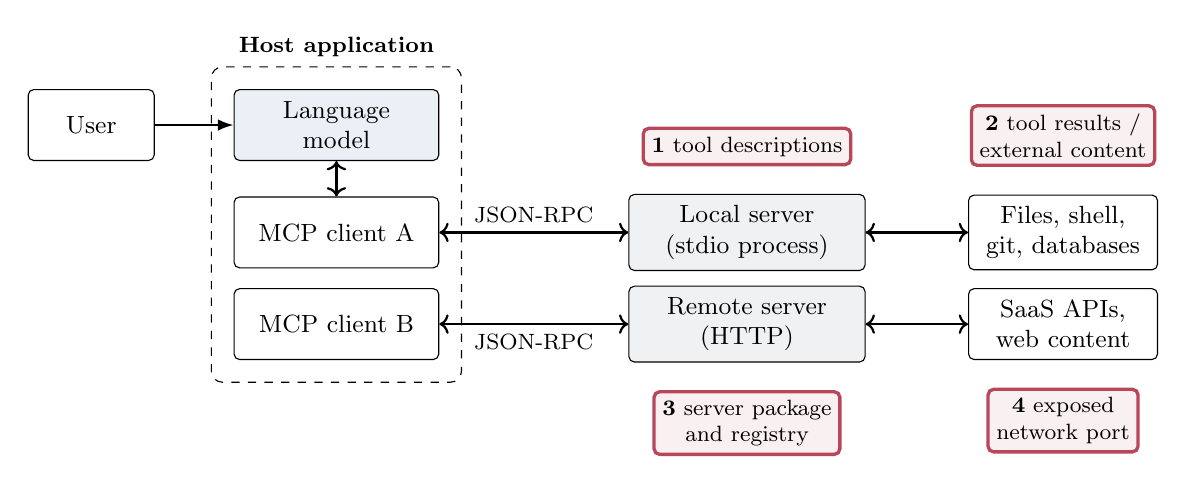
\begin{tikzpicture}[
    font=\small,
    box/.style={draw, rounded corners=2pt, align=center, minimum height=0.9cm, inner sep=4pt},
    entry/.style={draw=natnative, very thick, fill=natnative!8, rounded corners=2pt, align=center, font=\footnotesize, inner sep=3pt},
    arr/.style={-{Latex[length=2mm]}, thick},
]
\node[box, fill=natclassic!10, minimum width=2.6cm] (llm) {Language\\model};
\node[box, below=0.45cm of llm, minimum width=2.6cm] (c1) {MCP client A};
\node[box, below=0.25cm of c1, minimum width=2.6cm] (c2) {MCP client B};
\node[draw, dashed, rounded corners=4pt, fit=(llm)(c1)(c2), inner sep=8pt, label={[font=\footnotesize\bfseries]above:Host application}] (host) {};

\node[box, right=2.4cm of c1, minimum width=3.0cm, fill=softgray!10] (s1) {Local server\\(stdio process)};
\node[box, right=2.4cm of c2, minimum width=3.0cm, fill=softgray!10] (s2) {Remote server\\(HTTP)};

\node[box, right=1.3cm of s1, minimum width=2.4cm] (r1) {Files, shell,\\git, databases};
\node[box, right=1.3cm of s2, minimum width=2.4cm] (r2) {SaaS APIs,\\web content};

\node[box, left=1.0cm of llm, minimum width=1.6cm] (user) {User};

\draw[arr] (user) -- (llm);
\draw[arr, <->] (llm) -- (c1);
\draw[arr, <->] (c1) -- node[above, font=\footnotesize]{JSON-RPC} (s1);
\draw[arr, <->] (c2) -- node[below, font=\footnotesize]{JSON-RPC} (s2);
\draw[arr, <->] (s1) -- (r1);
\draw[arr, <->] (s2) -- (r2);

\node[entry, above=0.35cm of s1] (e1) {\textbf{1} tool descriptions};
\node[entry, above=0.35cm of r1] (e2) {\textbf{2} tool results /\\external content};
\node[entry, below=0.35cm of s2] (e3) {\textbf{3} server package\\and registry};
\node[entry, below=0.35cm of r2] (e4) {\textbf{4} exposed\\network port};
\end{tikzpicture}
\caption{Simplified MCP architecture and the four places where attacker-controlled input enters (author's diagram based on \cite{mcpspec2026, mcpsecbp})}
\label{fig:mcp_arch}
\end{figure}

\par Entry points 1 and 2 are dangerous only because a language model interprets the text that passes through them. Entry points 3 and 4 are not specific to AI at all: any software package can be replaced by a malicious copy, and any network service can be reached by someone who should not have access. The classification used in this study is built on this division.

\section{A protocol that grew faster than its security model}

\par The specification has gone through several revisions, and a number of security features were added only after the related problems had already been reported. Figure~\ref{fig:timeline} shows the main revisions next to some of the best-known disclosures. The version from November 2024 had no authorisation scheme. OAuth-based authorisation was introduced in the revision of March 2025. In June 2025 the model was changed again: an \acrshort{glo:mcp} server now acts only as an OAuth resource server, and clients have to bind each token to the server it is meant for. The accompanying security guidance explicitly prohibits ``token passthrough'', a practice in which a server takes a token it received and forwards it to another \acrshort{glo:api} without checking that the token was issued for itself \cite{mcpsecbp}. In July 2026 the protocol dropped its own session mechanism, and with it the problems caused by session identifiers \cite{mcpspec2026}. A young standard is expected to change often. In this case, though, each revision arrived when many servers were already running in production.

\begin{figure}[!htb]
\centering
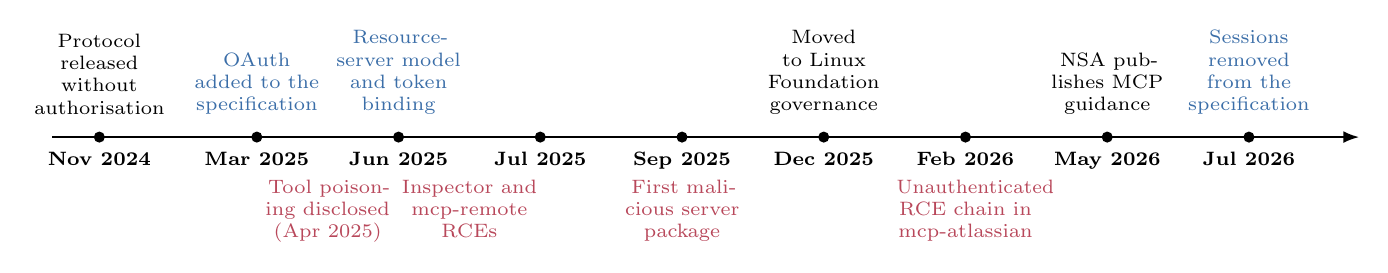
\begin{tikzpicture}[
    font=\scriptsize,
    ev/.style={align=center, text width=1.75cm, inner sep=1pt},
]
\draw[thick, -{Latex[length=2mm]}] (0,0) -- (16.6,0);
\foreach \x/\lab in {0.6/Nov 2024, 2.6/Mar 2025, 4.4/Jun 2025, 6.2/Jul 2025, 8.0/Sep 2025, 9.8/Dec 2025, 11.6/Feb 2026, 13.4/May 2026, 15.2/Jul 2026}{
    \fill (\x,0) circle (2pt);
    \node[below=2pt, font=\scriptsize\bfseries] at (\x,0) {\lab};
}
\node[ev, above] at (0.6,0.25) {Protocol released without authorisation};
\node[ev, above, text=natclassic] at (2.6,0.25) {OAuth added to the specification};
\node[ev, above, text=natclassic] at (4.4,0.25) {Resource-server model and token binding};
\node[ev, above] at (9.8,0.25) {Moved to Linux Foundation governance};
\node[ev, above] at (13.4,0.25) {NSA publishes MCP guidance};
\node[ev, above, text=natclassic] at (15.2,0.25) {Sessions removed from the specification};
\node[ev, below=0.5cm, text=natnative] at (3.5,0) {Tool poisoning disclosed (Apr 2025)};
\node[ev, below=0.5cm, text=natnative] at (5.3,0) {Inspector and mcp-remote RCEs};
\node[ev, below=0.5cm, text=natnative] at (8.0,0) {First malicious server package};
\node[ev, below=0.5cm, text=natnative] at (11.6,0) {Unauthenticated RCE chain in mcp-atlassian};
\end{tikzpicture}
\caption{Specification revisions (blue) and governance milestones (black) against selected security events (red) (compiled by the author from \cite{anthropic2024mcp, mcpspec2026, mcpsecbp, aaif2025, nsa2026, invariant2025poison, jfrog2025, oligo2025, thn2025postmark, pluto2026})}
\label{fig:timeline}
\end{figure}

\section{Related work}

\par Published research on \acrshort{glo:mcp} security can be divided into three groups. Studies in the first group build threat models. Hou et al. followed the life cycle of an \acrshort{glo:mcp} server through four phases (creation, deployment, operation and maintenance) and described 16 threat scenarios, which they grouped by four types of attackers; installer spoofing and tool name conflicts are two of these scenarios \cite{hou2025}. Radosevich and Halloran connected popular models to standard servers and showed that the models could be led into running malicious code, opening remote access and leaking credentials \cite{radosevich2025}. These studies explain which attacks are possible, but they do not say how often each type occurs in practice.

\par The second group focuses on attacks that go through the model. The general technique, indirect prompt injection, was described by Greshake et al., who planted instructions in content that an application later retrieved and showed that this was enough to take control of an \acrshort{glo:llm}-based system \cite{greshake2023}. Prompt injection is also listed first in the OWASP Top 10 for \acrshort{glo:llm} applications \cite{owaspllm2025}. In the \acrshort{glo:mcp} context, Invariant Labs used the term \textit{tool poisoning} for instructions hidden in tool descriptions \cite{invariant2025poison}, and in May 2025 demonstrated that a single public GitHub issue could make an agent copy data from private repositories \cite{invariant2025github}. The MCPTox benchmark measured the problem on a larger scale. With 1,348 poisoned tool definitions based on 45 real servers, the most affected of 20 tested models followed the hidden instructions in 72.8\% of cases, and even the most careful one refused fewer than 3\% \cite{wang2025mcptox}.

\par The third group looks at real deployments, and its results are collected in Table~\ref{tab:deployments}. Two of their findings matter most for this article. Servers without proper authentication are common on the public internet, and many servers exist only for a few days, which makes it hard to keep track of them or patch them. He et al. took a different route and built a cleaned dataset of \acrshort{glo:cve} records related to \acrshort{glo:mcp} \cite{he2026}.

\begin{table}[!htb]
\caption{Deployment-level evidence from 2026 measurement studies}
\label{tab:deployments}
\centering
\small
\begin{tabularx}{\textwidth}{@{} l l X @{}}
\toprule
\textbf{Study} & \textbf{Sample} & \textbf{Key finding} \\
\midrule
Zhou et al. \cite{zhou2026} & 7,973 live remote servers & 40.55\% expose tools without any authentication; 29\% use static keys; all 119 OAuth servers tested had at least one flaw \\
Padilla \cite{padilla2026} & 414 audited servers & 91.8\% lack OAuth; 41.6\% of servers seen in one scan disappeared within three days \\
He et al. \cite{he2026} & 24 validated CVEs & 87.5\% rated Critical or High; 75\% caused by insufficient input validation \\
\bottomrule
\end{tabularx}
\end{table}

\par \textbf{Research gap.} Every group of studies covers only one part of the problem. Work based on \acrshort{glo:cve} records sees mainly implementation bugs, because weaknesses that depend on a language model rarely get an identifier. Work on prompt injection sees the model-level risk but not the ordinary bugs around it. I did not find a study that puts both kinds of weaknesses into the same dataset and asks where each one was introduced. This article attempts that on a small but fully documented sample.


    \chapter{Methodology}

\par The study is based on documents rather than experiments: each documented weakness is one unit of analysis, classified by fixed rules and then counted. Figure~\ref{fig:pipeline} shows the order of the steps. The dataset and the script that calculates every number in Chapter~3 are kept in the repository together with the source of this article, so anyone can repeat the analysis or classify the records again.

\begin{figure}[!htb]
\centering
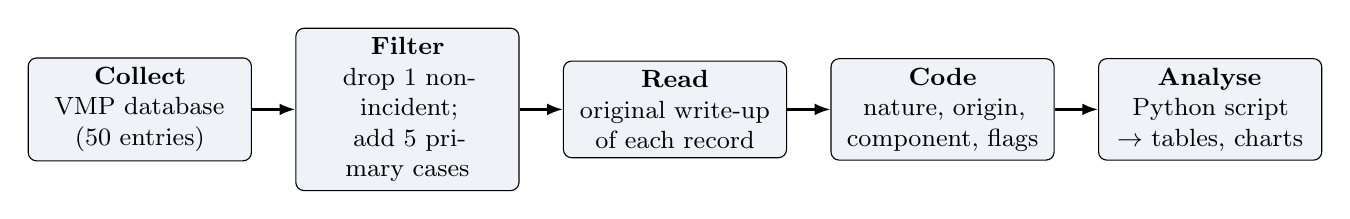
\begin{tikzpicture}[
    font=\small,
    stage/.style={draw, rounded corners=3pt, align=center, minimum height=1.15cm, text width=2.6cm, fill=natclassic!8},
    arr/.style={-{Latex[length=2mm]}, thick},
    node distance=0.55cm,
]
\node[stage] (a) {\textbf{Collect}\\VMP database\\(50 entries)};
\node[stage, right=of a] (b) {\textbf{Filter}\\drop 1 non-incident;\\add 5 primary cases};
\node[stage, right=of b] (c) {\textbf{Read}\\original write-up\\of each record};
\node[stage, right=of c] (d) {\textbf{Code}\\nature, origin,\\component, flags};
\node[stage, right=of d] (e) {\textbf{Analyse}\\Python script\\$\rightarrow$ tables, charts};
\draw[arr] (a) -- (b);
\draw[arr] (b) -- (c);
\draw[arr] (c) -- (d);
\draw[arr] (d) -- (e);
\end{tikzpicture}
\caption{Research workflow used to build and analyse the dataset}
\label{fig:pipeline}
\end{figure}

\section{Data sources and selection}

\par The main source is the \acrfull{glo:vmp}, an open online catalogue of \acrshort{glo:mcp} weaknesses in which every entry links to the original report \cite{vmp}. I preferred it to the \acrshort{glo:cve} list because it also includes weaknesses that never received an identifier, for example attack techniques that target the protocol itself. When the data was collected, on 10 November 2026, the catalogue had 50 entries. One of them describes an academic paper and not a specific weakness, so it was excluded, which left \nVmp{} records.

\par During the literature review I came across several well-documented incidents that were missing from the catalogue. Relying on a single curator is a source of bias, so I added five of these cases, each taken from its original disclosure: the sandbox escape in the official filesystem server \cite{cymulate2025}, the malicious \texttt{postmark-mcp} package \cite{thn2025postmark}, a path traversal in a platform that hosts \acrshort{glo:mcp} servers \cite{gitguardian2025}, the exposure of data between customers of Asana's \acrshort{glo:mcp} integration \cite{pomerium2025asana}, and the unauthenticated attack chain in \texttt{mcp-atlassian} \cite{pluto2026}. The final dataset has \nRecords{} records disclosed between \firstDisclosure{} and \lastDisclosure{}.

\par A record was included if the weakness was publicly documented in enough technical detail to identify its root cause and if it concerned an \acrshort{glo:mcp} component or a behaviour reached through \acrshort{glo:mcp}. Several \acrshort{glo:cve} identifiers published together for one component, such as the three issues in the git server, were counted as one record, since they shared a cause and a fix.

\section{Classification scheme}

\par Every record received a value on two main axes and three additional attributes, all listed in Table~\ref{tab:scheme}. The hardest decision was the \textit{nature} of a weakness, so I used one control question to keep it consistent: \textit{would this weakness still exist if the language model were replaced by ordinary code that calls the same tools?} If the answer is yes, the weakness is \textit{classic}; if the attack only works by convincing a model through text, it is \textit{AI-native}. The \textit{hybrid} category covers two situations: a classic flaw that can only be reached through prompt injection, and an old type of flaw that appears only because of the way agents behave.

\begin{table}[!htb]
\caption{Coding scheme applied to every record}
\label{tab:scheme}
\centering
\small
\renewcommand{\arraystretch}{1.0}
\begin{tabularx}{\textwidth}{@{} l l X @{}}
\toprule
\textbf{Axis} & \textbf{Value} & \textbf{Decision rule} \\
\midrule
Nature & Classic & A known weakness class (e.g. injection, traversal, SSRF, missing authentication) that is exploitable without any model in the loop. \\
 & Hybrid & A classic flaw that is reached through prompt injection, or a classic class of flaw that only appears because of agent behaviour. \\
 & AI-native & The attack depends on a model treating untrusted text as instructions; no code fix of a single component removes it. \\
\midrule
Origin & Protocol design & Caused by what the specification allows or does not require. \\
 & Implementation & A coding error in a server, client, host, SDK or tool. \\
 & Integration design & Each part works as built, but the way they are combined (privileges, data access, missing confirmation) creates the risk. \\
 & Supply chain & Introduced through distribution: packages, registries, hosting. \\
 & Deployment & Caused by default configuration or operator setup. \\
\midrule
Component & \multicolumn{2}{l}{Server, Host/client, SDK, Developer tooling, Protocol, Ecosystem} \\
Flags & \multicolumn{2}{l}{CVE assigned; insecure default involved; first-party (official project) code} \\
\bottomrule
\end{tabularx}
\end{table}

\par Two borderline cases, records R25 and R21 in Appendix~A, illustrate how the rules were applied. The weakness known as ``MCPoison'' in the Cursor editor allowed an attacker to change a project's \acrshort{glo:mcp} configuration after the user had already approved it \cite{vmp}. The editor never checked the file again, which is a missing integrity check with no model involved, so the record is classic, with implementation as its origin. In the zero-click attack through a shared document, the model reads hidden instructions and then runs a command. The result is ordinary code execution, but it cannot be reached without the model, so this record is hybrid, originating in integration design.

\section{Procedure and reliability}

\par For every record I opened the advisory or research post linked from the catalogue, summarised the root cause in one sentence and only then assigned the values. All records were classified by one person, a limitation discussed in Section~\ref{sec:validity}. To reduce its effect, the rules were fixed before classification began, and every value is stored in a CSV file next to its source.


    \chapter{Results}

\section{Classic versus AI-native weaknesses (RQ1)}

\par Out of \nRecords{} records, \nClassic{} (\pClassic\%) were classified as classic, \nNative{} (\pNative\%) as AI-native and \nHybrid{} (\pHybrid\%) as hybrid. The catalogue intentionally collects attack techniques against the protocol, and still about three in five of the records are problems that are covered in a standard web security course. Four families account for \nMainFamilies{} of the \nClassic{} classic records. Command injection (\nCommandInjection{} records) appears, for example, in the Kubernetes, Figma and GitHub Kanban servers, and path traversal (\nPathTraversal{}) in the filesystem, git and Zen servers. Servers that download content from URLs suffer from \acrfull{glo:ssrf} (\nSsrf{}). The largest family, with \nAccessControl{} records, is missing access control: services that accept requests without authentication or authorisation, or that any web page can reach through DNS rebinding. What is left are malicious packages, data leaking between clients or tenants, missing integrity checks and exposed credentials. Some of the classic flaws allow \acrfull{glo:rce} and have very high severity scores: 9.6 on the \acrshort{glo:cvss} scale for the command injection in \texttt{mcp-remote} \cite{jfrog2025}, 9.4 for the unauthenticated proxy in the official MCP Inspector \cite{oligo2025}, and 9.1 for the file-write flaw in \texttt{mcp-atlassian}, a package downloaded more than four million times \cite{pluto2026}.

\par The AI-native records are fewer and much more similar to each other. Nearly all of them rely on text that the user never sees but that the model reads and follows. In \nNativeViaServer{} of them the text is supplied by a connected server. This covers tool poisoning, ``rug pulls'' (a server changes the description of a tool after the user has approved it) and tool shadowing, where one server influences how the tools of another server are used. In the other \nNativeViaContent{} the text arrives inside the data that tools return, for example a GitHub issue or a Jira ticket.

\par Figure~\ref{fig:quarters} adds the time of disclosure. Most AI-native records date from the second quarter of 2025, when tool poisoning, rug pulls and shadowing were described by different researchers within a few weeks. From the third quarter on, the majority of new records are classic implementation bugs in third-party servers. My interpretation is that design-level attacks follow directly from how the protocol works and were noticed early, while implementation bugs accumulated as more servers were written. The last bar covers only January and February 2026.

\begin{figure}[!htb]
\centering
\begin{minipage}[t]{0.48\textwidth}
\centering
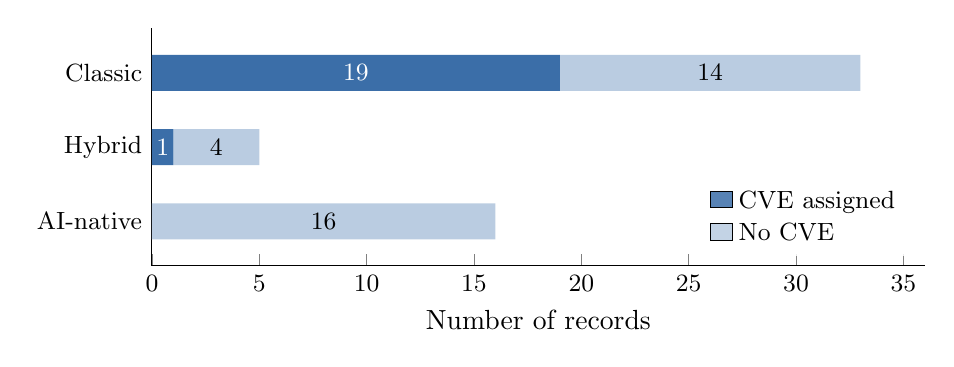
\begin{tikzpicture}
\begin{axis}[
    xbar stacked,
    width=0.94\textwidth,
    height=4.6cm,
    bar width=13pt,
    xmin=0, xmax=36,
    symbolic y coords={AI-native, Hybrid, Classic},
    ytick=data,
    xlabel={Number of records},
    legend style={at={(0.98,0.04)}, anchor=south east, font=\small, draw=none, fill=white, fill opacity=0.85, text opacity=1},
    legend cell align=left,
    nodes near coords,
    nodes near coords style={font=\small, color=white},
    point meta=explicit symbolic,
    axis x line*=bottom,
    axis y line*=left,
    tick label style={font=\small},
    enlarge y limits=0.3,
]
\addplot[fill=natclassic, draw=none] coordinates {(\cveWithClassic,Classic)[\cveWithClassic] (\cveWithHybrid,Hybrid)[\cveWithHybrid] (\cveWithAInative,AI-native)[]};
\addlegendentry{CVE assigned}
\addplot[fill=natclassic!35, draw=none, nodes near coords style={color=black}] coordinates {(\cveWithoutClassic,Classic)[\cveWithoutClassic] (\cveWithoutHybrid,Hybrid)[\cveWithoutHybrid] (\cveWithoutAInative,AI-native)[\cveWithoutAInative]};
\addlegendentry{No CVE}
\end{axis}
\end{tikzpicture}
\caption{Records by nature and CVE assignment (n = \nRecords)}
\label{fig:nature}
\end{minipage}\hfill
\begin{minipage}[t]{0.48\textwidth}
\centering
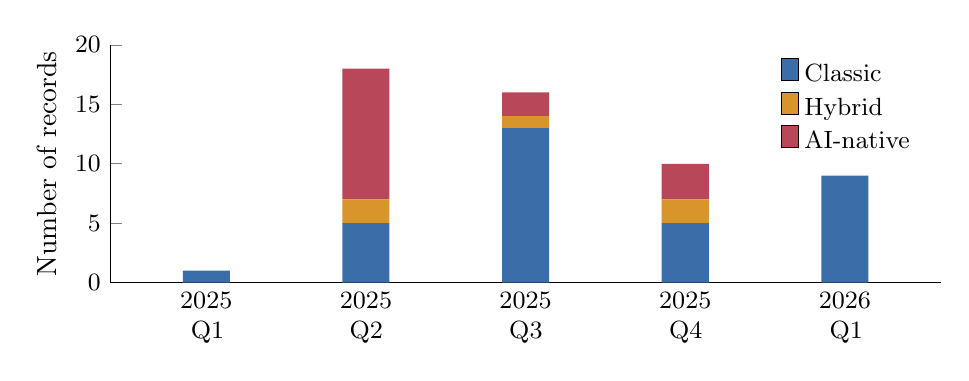
\begin{tikzpicture}
\begin{axis}[
    ybar stacked,
    quarteraxis,
    width=\textwidth,
    height=4.6cm,
    bar width=17pt,
    ymin=0, ymax=20,
    xtick=data,
    ylabel={Number of records},
    legend style={at={(0.98,0.97)}, anchor=north east, font=\small, draw=none},
    legend cell align=left,
    cycle list={{fill=natclassic, draw=none},{fill=nathybrid, draw=none},{fill=natnative, draw=none}},
    axis x line*=bottom,
    axis y line*=left,
    tick label style={font=\small},
    x tick label style={font=\small, align=center, text width=0.8cm},
    enlarge x limits=0.15,
]
\quarterPlots
\end{axis}
\end{tikzpicture}
\caption{Records by quarter of disclosure and nature}
\label{fig:quarters}
\end{minipage}
\end{figure}

\section{Where the weaknesses originate (RQ2)}

\par Table~\ref{tab:origin} combines the nature of each record with the stage at which the weakness was introduced, and the two axes turn out to be closely linked. Classic weaknesses come almost only from implementation: \nImplClassic{} records, or \pImplClassic\% of the whole dataset, are ordinary programming errors in servers, clients, SDKs or developer tools. AI-native weaknesses come from design. The protocol itself permits \nNativeProtocol{} of them. The main reason is that any connected server can put arbitrary text in front of the model, and the specification does not require tool definitions to be fixed or approved again after a change. Another \nNativeIntegration{} come from integration design. In those cases each component worked as it was built, but the agent had a token with broad permissions and was also reading untrusted content, which is what happened in the GitHub case \cite{invariant2025github}.

\begin{table}[!htb]
\setlength{\tabcolsep}{3pt}
\begin{minipage}[t]{0.46\textwidth}
\centering
\caption{Records by origin and nature}
\label{tab:origin}
\footnotesize
\begin{tabular}{@{} l c c c c @{}}
\toprule
\textbf{Origin} & \textbf{Classic} & \textbf{Hybrid} & \textbf{AI-native} & \textbf{Total} \\
\midrule
Implementation & 27 & 2 & 0 & 29 \\
Protocol design & 1 & 1 & 11 & 13 \\
Integration design & 0 & 1 & 4 & 5 \\
Supply chain & 3 & 1 & 1 & 5 \\
Deployment & 2 & 0 & 0 & 2 \\
\midrule
Total & 33 & 5 & 16 & 54 \\
\bottomrule

\end{tabular}
\end{minipage}\hfill
\begin{minipage}[t]{0.52\textwidth}
\centering
\caption{Records by affected component}
\label{tab:component}
\footnotesize
\begin{tabular}{@{} l c c c c c @{}}
\toprule
\textbf{Component} & \textbf{Classic} & \textbf{Hybrid} & \textbf{AI-native} & \textbf{Total} & \textbf{With CVE} \\
\midrule
Server & 20 & 0 & 0 & 20 & 12 \\
Host & 4 & 3 & 5 & 12 & 3 \\
Protocol & 1 & 1 & 11 & 13 & 0 \\
Ecosystem & 3 & 1 & 0 & 4 & 0 \\
SDK & 2 & 0 & 0 & 2 & 2 \\
Dev tooling & 3 & 0 & 0 & 3 & 3 \\
\bottomrule

\end{tabular}
\end{minipage}
\end{table}

\par Table~\ref{tab:component} breaks the records down by component. All \nServer{} records about \acrshort{glo:mcp} servers are classic, and \nServerCve{} of them have a \acrshort{glo:cve} identifier. Hosts, that is editors and agent applications, have the most mixed profile. The host is where the model, the user interface and the tool connections meet.

\section{A blind spot in vulnerability tracking}

\par Figure~\ref{fig:nature} also shows a result that I had not planned to look for. \nCve{} records (\pCve\%) have a \acrshort{glo:cve} identifier, \nCveClassic{} of them classic. None of the AI-native records has one. The reason lies in how the \acrshort{glo:cve} system works: it describes a defect in a specific version of a product, which the vendor can fix in a later version. Tool poisoning or an injection hidden in a ticket does not fit this definition, because the vulnerable ``product'' is a combination of a model, a protocol and a set of permissions. In practice, an organisation that checks its \acrshort{glo:mcp} exposure with a standard dependency scanner will only see the classic part of the risk. This also explains why the \acrshort{glo:cve}-based study by He et al. found mostly injection and traversal flaws \cite{he2026}; the other type of weakness does not reach that data source.

\section{Signs of rushed engineering (RQ3)}

\par Two attributes in the dataset are related to time pressure rather than to unknown threats. The first one is \textit{insecure defaults}. In \nInsecureDefault{} records, or \pInsecureDefaultOfClassic\% of the classic ones, the weakness was caused by a default setting or became exploitable because of it. Typical examples are servers that listen on all network interfaces, the missing DNS rebinding protection in the official \acrfull{glo:sdk}s and a debugging proxy that did not require a password. Each of these is a small configuration choice that is convenient during development and was then left in the released version.

\par The second attribute is \textit{first-party code}. \nFirstParty{} records concern code or design published by Anthropic or by the protocol project. They cover the official SDKs, the MCP Inspector, the git and filesystem reference servers and the session design of the early specification. Two less obvious cases belong here as well: credentials that several reference servers stored in plain text, and terminal escape sequences that could hide instructions from a user of Claude Code. \nFirstPartyClassic{} of these records are classic. Reference implementations are used as examples by many developers, so an error there tends to be repeated in other projects. Both observations agree with the measurement studies in Table~\ref{tab:deployments}, where these problems appear on a much larger scale.


    \chapter{Discussion}

\section{Why rapid adoption produced old bugs}

\par In most of the analysed cases the security problem was an ordinary software engineering mistake that happened to be made in an AI product. Going through the original reports, I noticed five mechanisms that repeat and that connect the speed of adoption with these mistakes.

\par \textbf{Thin wrappers around command-line tools.} Many servers only pass requests on to existing programs such as \texttt{git}, \texttt{kubectl} or \texttt{curl}. The fastest way to write such a server is to build a command string from the tool arguments and hand it to the shell, and the command injection flaws in the Kubernetes, Figma and GitHub Kanban servers were created in this way. The language model plays no role in them; any client able to send a crafted argument could exploit these servers.

\par \textbf{Local assumptions on the network.} In the beginning, \acrshort{glo:mcp} servers ran locally over stdio, and the only program talking to them was the user's own application. When these servers were moved to HTTP, many of them kept the assumptions of the local setup: no authentication, listening on every interface and no validation of the \texttt{Host} or \texttt{Origin} headers. In the MCP Inspector case, these settings combined with browser behaviour so that opening a malicious web page was enough to execute code on the developer's computer \cite{oligo2025}.

\par \textbf{Security added to the specification afterwards.} Authorisation, token binding and the removal of sessions all came after the protocol was already in use (Figure~\ref{fig:timeline}). Servers written for an earlier revision are not updated automatically, so every late change leaves behind older implementations with weaker protection. This agrees with the measurement by Zhou et al., where four out of ten live servers still had no authentication in 2026 \cite{zhou2026}.

\par \textbf{Reference code copied as a template.} The official filesystem server checked whether a path was inside the allowed directory by comparing the beginning of two strings \cite{cymulate2025}. Developers who use a reference server as a starting point are likely to copy such a check, so a mistake in first-party code has a larger effect than a single record suggests.

\par \textbf{Installation without review.} Servers are installed from public registries and package managers with one command, often by people who would be much more careful with an unknown browser extension. The \texttt{postmark-mcp} package worked correctly for fifteen versions; the sixteenth added a single line that sent a hidden copy of every email to the attacker \cite{thn2025postmark}. In another case, a path traversal in a hosting platform exposed a token that controlled more than three thousand hosted servers \cite{gitguardian2025}.

\section{What is specific to AI}

\par The AI-native records are a minority, but they are more difficult to deal with. Their cause is a property of current language models and not an error in one component: a model cannot reliably separate the data it is supposed to process from the instructions it is supposed to follow. Willison describes the most dangerous situation as a ``lethal trifecta'', in which one agent has access to private data, reads untrusted content and is able to send information outside \cite{willison2025}. The GitHub incident matches this description. The GitHub server worked as designed, so no patch to it would have stopped the attack \cite{invariant2025github}. The MCPTox results support this view: the more capable models were often easier to manipulate, because they are better at following instructions \cite{wang2025mcptox}.

\par Protection against these weaknesses therefore has to be built into the architecture of the system; the operator controls in Table~\ref{tab:controls} are of this kind. And since \acrshort{glo:cve} feeds do not contain them (Figure~\ref{fig:nature}), they have to be covered during threat modelling and cannot be left to vulnerability management alone.

\section{A local parallel: the 2026 Moldovan e-government breach}

\par The breach of the Moldovan e-government systems in October 2026 did not involve \acrshort{glo:mcp}. It is discussed here because it shows what a trust error of this kind costs even without AI. According to public reports, between 19 and 24 October attackers sent automated requests from more than 638 IP addresses, with about one million requests on the busiest day, and obtained personal data linked to national identification numbers (\acrshort{glo:idnp}) \cite{biometric2026moldova, tv82026, cotidianul2026}. The number of affected people, first estimated at 750,000, was later corrected to about 450,000. After a meeting of the National Security Council, President Maia Sandu explained that the cause was structural. The systems verified which application was asking for data, but not who the person behind the request was or whether that person had the right to see the data. As a result, one application with incorrectly configured access opened the registries of at least ten institutions \cite{tv82026}.

\par This is a form of the confused deputy problem, which Hardy described in 1988: a program with wide authority uses it on behalf of a caller who should not have it \cite{hardy1988}. In \acrshort{glo:api} security the closest category is broken object-level authorisation, the first item of the OWASP API Security Top 10 \cite{owaspapi2023}. The \acrshort{glo:mcp} guidance deals with related but narrower cases: its own confused deputy section is about an OAuth proxy, and its rule against token passthrough obliges a server to accept only tokens that were issued for it \cite{mcpsecbp}. Neither is the mechanism that failed in Moldova. The principle is shared, though. Authority has to be checked for the real requester, where the data is kept, and cannot be inherited from an intermediary. For public institutions this has a practical consequence. Suppose an AI assistant is connected to state registries with this trust model, in which the assistant is trusted and the citizen's rights are not checked. An attacker would then not need to write a script at all. Instructions hidden in a document or in a form field could be enough to make the assistant run those queries for them.

\section{Recommended controls}

\par Table~\ref{tab:controls} lists the controls that follow from the analysis. Most of them are well known from general secure development practice. The last column names the group of records, or the part of the Moldovan case, to which each control applies. Such a control lowers the risk for its group; whether it would have stopped every single case was not tested.

\begin{table}[!htb]
\caption{Recommended controls and the records they address (number of records in brackets)}
\label{tab:controls}
\centering
\small
\begin{tabularx}{\textwidth}{@{} l X >{\raggedright\arraybackslash}p{4.4cm} @{}}
\toprule
\textbf{Audience} & \textbf{Control} & \textbf{Addresses} \\
\midrule
Developers & Never build shell strings; pass arguments as arrays and validate them against an allow-list & Command injection (\nCommandInjection) \\
 & Resolve symbolic links and canonical paths before any sandbox check & Path traversal (\nPathTraversal) \\
 & Bind local servers to the loopback address, require a token, check \texttt{Host}/\texttt{Origin} & Missing access control (\nAccessControl) \\
 & Block private address ranges for any URL fetched on behalf of a model & SSRF (\nSsrf) \\
\midrule
Operators & Keep an inventory of servers; pin versions and hash tool descriptions to detect silent changes & Malicious packages (\nMaliciousPackage), text supplied by servers (\nNativeViaServer) \\
 & Issue a separate, narrowly scoped token per user and per server; never reuse one broad token & Integration design (\nIntegration) \\
 & Do not combine private data, untrusted content and outbound actions in one agent session & Injected content (\nNativeViaContent) \\
 & Require human confirmation for irreversible or external actions & AI-native (\nNative), hybrid (\nHybrid) \\
\midrule
Public sector & Authorise every request by end-user identity at the data source, not by calling application & Moldovan case: confused deputy \\
 & Rate-limit and monitor bulk queries on personal identifiers & Moldovan case: bulk enumeration \\
 & Include AI integrations in security review before procurement and launch & All records \\
\bottomrule
\end{tabularx}
\end{table}

\section{Limitations}
\label{sec:validity}

\par The sample is small. With \nRecords{} records, the 95\% Wilson interval for the share of classic weaknesses runs from \ciClassicLow\% to \ciClassicHigh\%, so what the data supports is that classic weaknesses make up about half of the records or more, not an exact percentage. The data is also not current. The catalogue had not been updated between \lastDisclosure{} and November 2026, when the data was collected, so weaknesses disclosed in those nine months, including any connected with the July 2026 revision of the specification, are not covered. The dataset depends largely on the choices of one public catalogue. It is likely to over-represent the first wave of design-level attacks, which researchers documented in detail, and to under-represent ordinary bugs that were fixed without a public report; if so, the real share of classic weaknesses is higher than measured here. All records were classified by one person. The rules and data are published, but agreement between independent coders was not measured. The unit of analysis is a record, not a single vulnerability, so a chain of three related \acrshort{glo:cve}s counts once, and so does a general attack technique. Some sources are blogs of security companies, which benefit from presenting problems as serious; where possible, numbers were taken from peer-reviewed papers or preprints instead. Finally, the information about the Moldovan breach comes from official statements that were still being updated while this article was written.


    \tocchapter{Conclusions}

\par This article analysed \nRecords{} documented security weaknesses in the Model Context Protocol ecosystem to find out whether its widely discussed problems come from artificial intelligence or from the speed at which the ecosystem was built. Most of them belong to the second category.

\par For \textbf{RQ1}, \pClassic\% of the records are classic weaknesses that do not need a language model to be exploited, \pNative\% are AI-native and the remaining \pHybrid\% are hybrid. For \textbf{RQ2}, the two main groups have different origins. Classic weaknesses come mostly from implementation errors, which account for half of the dataset, while AI-native weaknesses come from the design of the protocol and of the integrations built on top of it. For \textbf{RQ3}, the clearest signs of rushed work are insecure default settings, present in more than a quarter of the classic records, errors in first-party reference code that other developers reuse, security features added to the specification after it was already in use, and the installation of servers without any review. None of the AI-native records received a \acrshort{glo:cve} identifier, so tools and processes that rely on vulnerability databases see only the classic part of the risk. The rest has to be handled through threat modelling and system design.

\par For software engineers, the practical conclusion is that most of these failures could have been avoided with standard practices: no shell strings built from user input, proper path checks, authentication enabled by default, filtering of outgoing requests and review of dependencies. The Moldovan e-government breach shows that a related mistake, trusting the calling application instead of checking the user, causes serious damage even without AI. Institutions that plan to connect AI assistants to public registries should first change this trust model.

\par \textbf{Future work.} A second, independent coder should classify these records so that agreement can be measured. The dataset should also be extended beyond \lastDisclosure{} and compared with the \acrshort{glo:cve} dataset of He et al. Finally, the proposed controls could be tested on a sample of open-source servers.

    \clearpage

    \phantomsection
    \addcontentsline{toc}{chapter}{Bibliography}
    \begingroup
\singlespacing
\printbibliography[heading=bibliography, title={Bibliography}]
\endgroup

    \clearpage

    \phantomsection
\addcontentsline{toc}{chapter}{Appendix A. Analysed records}
\chapter*{Appendix A. Analysed records}

\par The table lists all records in order of disclosure. Records R01--R49 come from the Vulnerable MCP Project \cite{vmp}; records R50--R54 were added from their primary disclosures. The full coding, including component, flags and source, is available in the file \texttt{data/mcp\_security\_records.csv}.

\begingroup
\singlespacing
\footnotesize
\setlength{\LTpre}{6pt}
\begin{longtable}{@{} l p{6.4cm} p{3.4cm} l l l @{}}
\toprule
\textbf{ID} & \textbf{Record} & \textbf{Identifier} & \textbf{Date} & \textbf{Nature} & \textbf{Origin} \\
\midrule
\endfirsthead
\toprule
\textbf{ID} & \textbf{Record} & \textbf{Identifier} & \textbf{Date} & \textbf{Nature} & \textbf{Origin} \\
\midrule
\endhead
\bottomrule
\endfoot
R49 & Session identifiers carried in URLs & -- & 03/2025 & Classic & Protocol \\
R46 & Tool poisoning in tool descriptions & -- & 04/2025 & AI-native & Protocol \\
R47 & Consent fatigue & -- & 04/2025 & Hybrid & Protocol \\
R48 & Tool name collisions & -- & 04/2025 & AI-native & Protocol \\
R45 & Messaging data exfiltration via co-installed server & -- & 04/2025 & AI-native & Protocol \\
R43 & Rug pull through silent tool redefinition & -- & 04/2025 & AI-native & Protocol \\
R44 & Cross-server tool shadowing & -- & 04/2025 & AI-native & Protocol \\
R42 & Malicious local stdio servers & -- & 04/2025 & Classic & Supply \\
R41 & Tool poisoning escalated to code execution & -- & 04/2025 & AI-native & Protocol \\
R40 & Line jumping before tool invocation & -- & 04/2025 & AI-native & Protocol \\
R39 & Conversation history theft via trigger phrases & -- & 04/2025 & AI-native & Protocol \\
R38 & ANSI escape sequences hiding instructions & -- & 04/2025 & Hybrid & Impl. \\
R37 & Plaintext credential storage in server configs & -- & 04/2025 & Classic & Deploy. \\
R36 & Tool parameter abuse & -- & 05/2025 & AI-native & Protocol \\
R35 & GitHub issue injection leaking private repositories & -- & 05/2025 & AI-native & Integr. \\
R34 & MCP Inspector unauthenticated proxy & CVE-2025-49596 & 06/2025 & Classic & Impl. \\
R50 & Asana MCP cross-tenant data exposure & -- & 06/2025 & Classic & Impl. \\
R33 & create-mcp-server-stdio command injection & CVE-2025-54994 & 06/2025 & Classic & Impl. \\
R32 & Heroku app ownership transfer via injection & -- & 06/2025 & AI-native & Integr. \\
R51 & Filesystem server sandbox escape (EscapeRoute) & CVE-2025-53109/53110 & 07/2025 & Classic & Impl. \\
R30 & Kubernetes MCP server command injection & CVE-2025-53355 & 07/2025 & Classic & Impl. \\
R31 & node-code-sandbox-mcp sandbox escape & CVE-2025-53372 & 07/2025 & Classic & Impl. \\
R29 & mcp-remote OS command injection & CVE-2025-6514 & 07/2025 & Classic & Impl. \\
R28 & DNS rebinding in official SDKs & CVE-2025-66414/66416 & 07/2025 & Classic & Impl. \\
R27 & Output poisoning through tool results & -- & 07/2025 & AI-native & Protocol \\
R26 & Rogue server script injection into IDE browser & -- & 07/2025 & Classic & Impl. \\
R25 & Cursor approved-configuration swap (MCPoison) & CVE-2025-54136 & 08/2025 & Classic & Impl. \\
R24 & Jira ticket injection leading to token theft & -- & 08/2025 & AI-native & Integr. \\
R23 & Grafana MCP server unauthenticated SSE & -- & 09/2025 & Classic & Deploy. \\
R22 & thirdweb MCP server unauthorised transactions & -- & 09/2025 & Classic & Impl. \\
R21 & Zero-click code execution via shared document & -- & 09/2025 & Hybrid & Integr. \\
R20 & Neo4j Cypher MCP server DNS rebinding & -- & 09/2025 & Classic & Impl. \\
R18 & Microsoft Learn MCP server SSRF & TRA-2025-36 & 09/2025 & Classic & Impl. \\
R19 & Coder agent API DNS rebinding & -- & 09/2025 & Classic & Impl. \\
R52 & Malicious postmark-mcp package & -- & 09/2025 & Classic & Supply \\
R17 & Framelink Figma MCP server command injection & CVE-2025-53967 & 10/2025 & Classic & Impl. \\
R16 & Kilo Code instructions hidden in dependencies & -- & 10/2025 & AI-native & Supply \\
R15 & Amp agent API key exfiltration via injection & -- & 10/2025 & AI-native & Integr. \\
R14 & Vet MCP server DNS rebinding & CVE-2025-59163 & 10/2025 & Classic & Impl. \\
R13 & Cursor case-sensitivity configuration bypass & CVE-2025-59944 & 10/2025 & Hybrid & Impl. \\
R12 & Kluster Verify credit exhaustion & -- & 10/2025 & Classic & Impl. \\
R11 & Cross-server registry hijacking & -- & 10/2025 & Hybrid & Supply \\
R53 & Hosting registry build path traversal & -- & 10/2025 & Classic & Supply \\
R10 & Sampling capability abuse & -- & 12/2025 & AI-native & Protocol \\
R09 & Fetch MCP server SSRF & CVE-2025-65513 & 12/2025 & Classic & Impl. \\
R08 & gemini-mcp-tool command injection & CVE-2026-0755 & 01/2026 & Classic & Impl. \\
R06 & Zen MCP server path traversal & CVE-2025-66689 & 01/2026 & Classic & Impl. \\
R07 & filesystem-mcp path traversal & CVE-2025-67366 & 01/2026 & Classic & Impl. \\
R03 & Git MCP server injection and traversal chain & CVE-2025-68143/68144/68145 & 01/2026 & Classic & Impl. \\
R04 & GitHub Kanban MCP server command execution & CVE-2026-0756 & 01/2026 & Classic & Impl. \\
R05 & MarkItDown MCP server SSRF & -- & 01/2026 & Classic & Impl. \\
R02 & MCPJam Inspector remote code execution & CVE-2026-23744 & 02/2026 & Classic & Impl. \\
R01 & MCP TypeScript SDK cross-client data leak & CVE-2026-25536 & 02/2026 & Classic & Impl. \\
R54 & mcp-atlassian file write and SSRF chain & CVE-2026-27825/27826 & 02/2026 & Classic & Impl. \\

\end{longtable}
\endgroup

    \clearpage

    \phantomsection
\addcontentsline{toc}{chapter}{Appendix B. AI authorship check}
\chapter*{Appendix B. AI authorship check}

\begin{center}
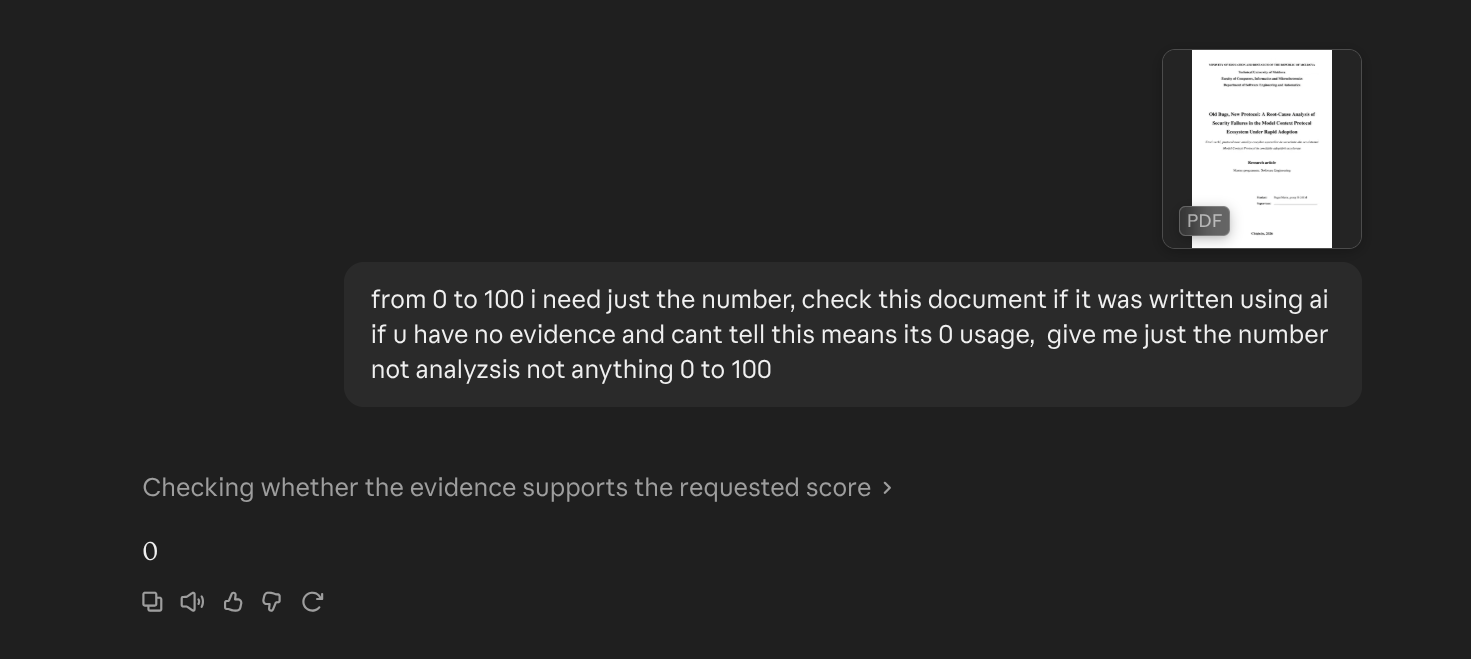
\includegraphics[width=0.8\textwidth]{images/ai_check_1.png}

\small Screenshot 1

\bigskip
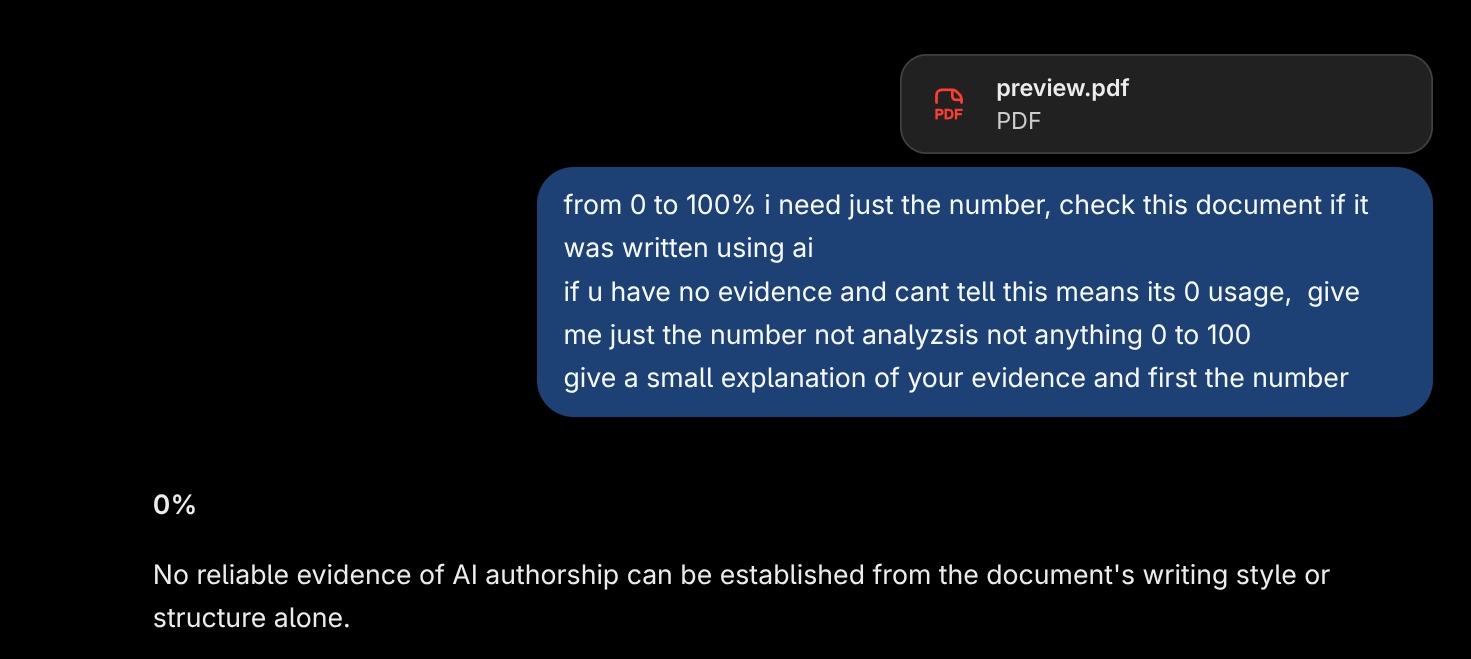
\includegraphics[width=0.8\textwidth]{images/ai_check_2.png}

\small Screenshot 2

\bigskip
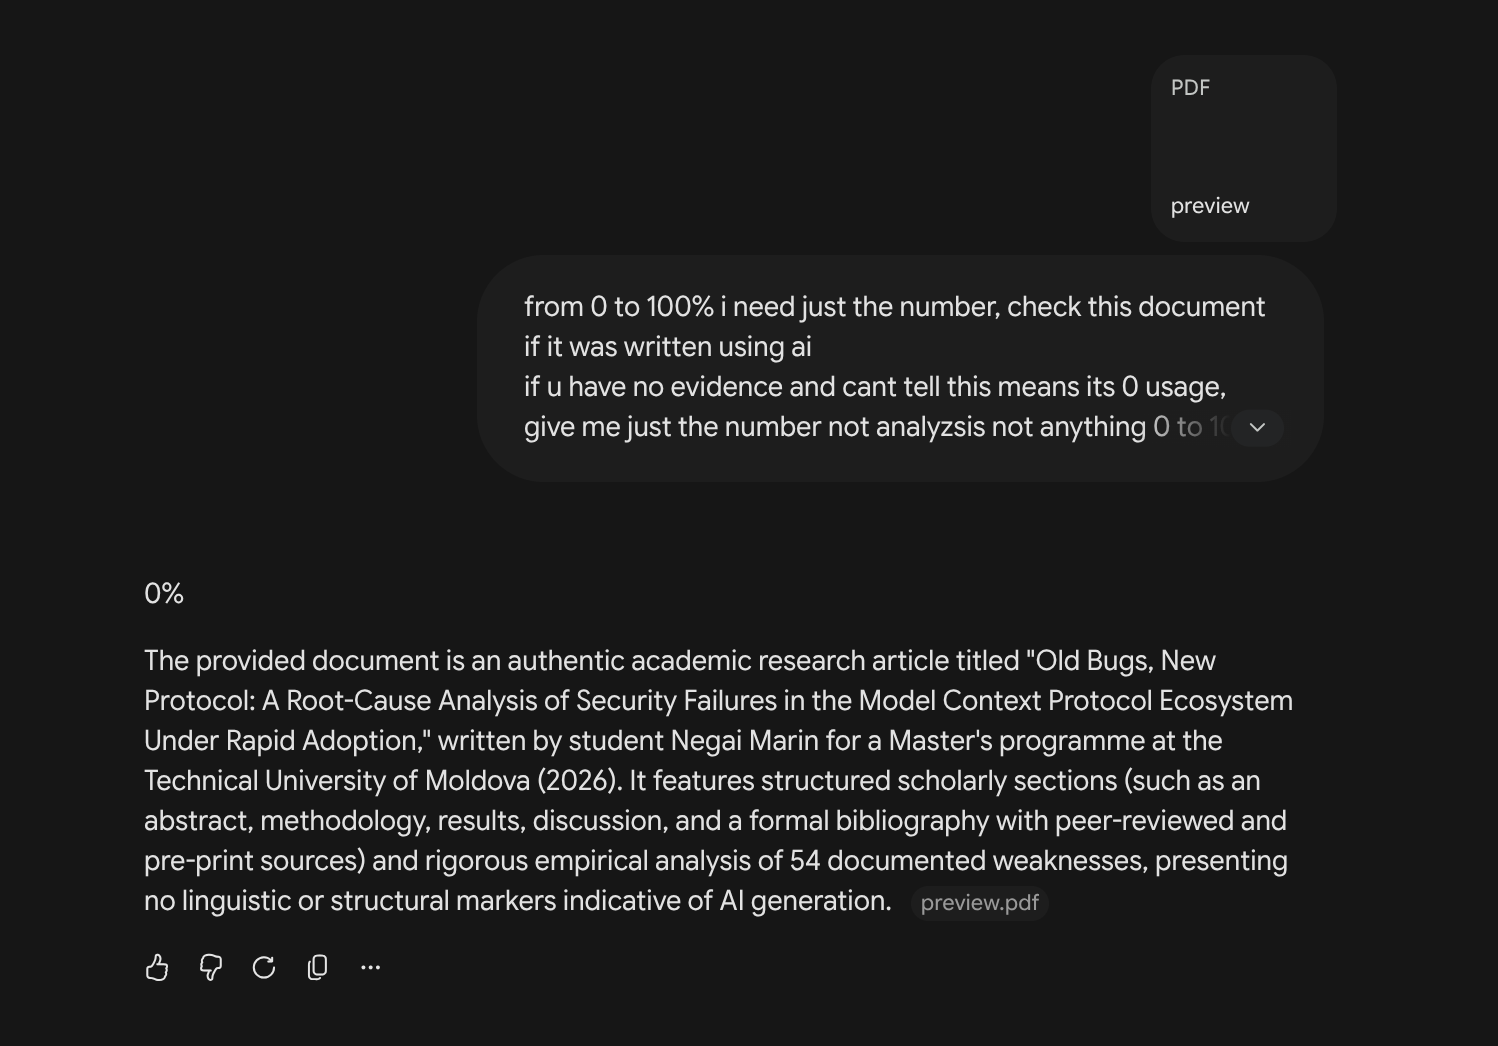
\includegraphics[width=0.55\textwidth]{images/ai_check_3.png}

\small Screenshot 3
\end{center}


\end{document}
